	Zeitordnungsoperator T : \marginpar{19.10.2015}
		\begin{align*}
		\T A(t_1) A(t_2) = 
		\left\{
			\begin{aligned}
				A(t_1) A(t_2) &, t_1 \geq t_2 \\
				A(t_2) A(t_1) &, t_1 \leq t_2 
			\end{aligned}
		\right.
		\end{align*}
		\begin{equation*}
			\Rightarrow \T A(t_1) A(t_2) \cdots A(t_k) = A(t_{\pi(1)}) A(t_{\pi(2)}) \cdots A(t_{\pi(k)})
		\end{equation*}
	mit $\pi \in S_k$ (Gruppe der Permutationen von k Elementen (mit Mächtigkeit $k!$))
	sodass wenn $t_{\pi(1)} \geq t_{\pi(2)} \geq \ldots \geq t_{\pi(k)}$
		\begin{align*}
			W(t) &= \T 
			\left\{
				\sum_{k=0}^\infty \left( \frac{-i}{\hbar}\right)^k \frac{1}{k!} 
				\int_{0}^{t} \diff t_k \int_{0}^{t} \diff t_{k-1} \cdots
				\int_{0}^{t} \diff t_1 
				H_W^1(t_k) H_W^1(t_{k-1}) \cdots H_W^1(t_1) \mathds{1} 
			\right\} \\
			&= \T
			\left\{\vphantom{\sum_{k=0}^{\infty}} \right.
				\sum_{k=0}^{\infty} 
				\left( \frac{-i}{\hbar}\right)^k \frac{1}{k!}
				\underbrace{
					\int_{0}^{t} \diff t_k H_W^1(t_k) 
					\int_{0}^{t} \diff t_{k-1} H_W^1(t_{k-1}) \cdots
					\int_{0}^{t} \diff t_1 H_W^1(t_1)
				}_{\mathclap{\left( \int_{0}^{t} \diff t' H_W^1(t') \right)^k }}
			\left. \vphantom{\sum_{k=0}^{\infty}}\right\} \\
			% bemerkung: mit \vphantom sind die klammern jetzt nicht mehr so riesig.
			&= \T \exp 
			\left\{
				- \frac{i}{\hbar} \int_{0}^{t} \diff t' H_W^1(t')
			\right\}
		\end{align*}
	mit
		\begin{align*}
			i\hbar \frac{\diff}{\diff t} \ket{\psi_W(t)} &= H_W^1(t) \ket{\psi_W(0)} \\
			\Rightarrow 
			\ket{\psi_W(t)} &= \T e^{-\frac{i}{\hbar} \int_{0}^{t} \diff t' H_W^1(t')} \ket{\psi(0)}
		\end{align*}
	Hier kommt ein mathematischer Einschub oder sowas (what so ever):
		\begin{align*}
			\int_{0}^{t} \diff t' \int_{0}^{t'} \diff t'' f(t') f(t'') 
			&= \int_{0}^{t} \diff t' 
			\left( \vphantom{\int_{0}^{t'} \diff t''} \right.
				\int_{0}^{t'} \diff t'' \underbrace{f(t')}_{\mathclap{t' > t''}} f(t'') 
				+ \int_{t'}^{t} \diff t'' \underbrace{f(t'')}_{\mathclap{t'' > t'}} f(t')
				\left. \vphantom{\int_{0}^{t'} \diff t''} 
			\right) 
			\frac{1}{2} \\
			\int_{0}^{t} \diff t' \int_{t'}^{t} \diff t'' f(t'') f(t') 
			&= \int_{0}^{t} \diff t'' \int_{0}^{t'} \diff t' f(t'') f(t') = \int_{0}^{t} \diff t' \int_{0}^{t'} \diff t'' f(t') f(t'') 
		\end{align*}	
	Die Übergangswahrscheinlichkeit vom Zustand $\ket{n}$ zur Zeit $t_0$ in den Zustand $\ket{m}$ zur Zeit $t>t_0$ lautet:
		\begin{align*}
			P_{mn} &= \left| c_m(t) \right|^2 \\
			&= \left| \braket{m | \psi_W(t)} \right|^2 \\
			&= \left| \braket{m | W(t,t_0) | \psi_W(t_0)} \right|^2 \\
			&= \left| \braket{m | W(t,t_0) | n}\right|^2
		\end{align*}
	Hier ist wieder $\ket{n} = \ket{\psi(t_0)}$.
\subsection{Fermis Goldene Regel}
	Betrachte zeitlich konstante Störung
		\begin{align*}
			H^1(t) &= \underbrace{\Theta (t)}_{\substack{Heaviside}} H^1 \\
		\end{align*}
	$\Rightarrow$ für $m \neq n$, 1.Ordnung Störungstheorie:
		\begin{align*}
			P_{mn}(t) 
			&= \frac{1}{\hbar^2} \left| \braket{m | H^1 | n}\right|^2 
			\cdot \left| \int_{0}^{t} \diff t' e^{-i(\omega_m-\omega_n) t'} \right|^2 \\
			&= \frac{4}{\hbar^2} \frac{\sin^2[(\omega_m-\omega_n)
			\frac{t_0}{2}]}{(\omega_m-\omega_n)^2} 
			\left| \braket{m | H^1 | n}\right|^2
		\end{align*}
	PLOT NUMMER 1
	\begin{figure*} [h]
		\begin{center}
			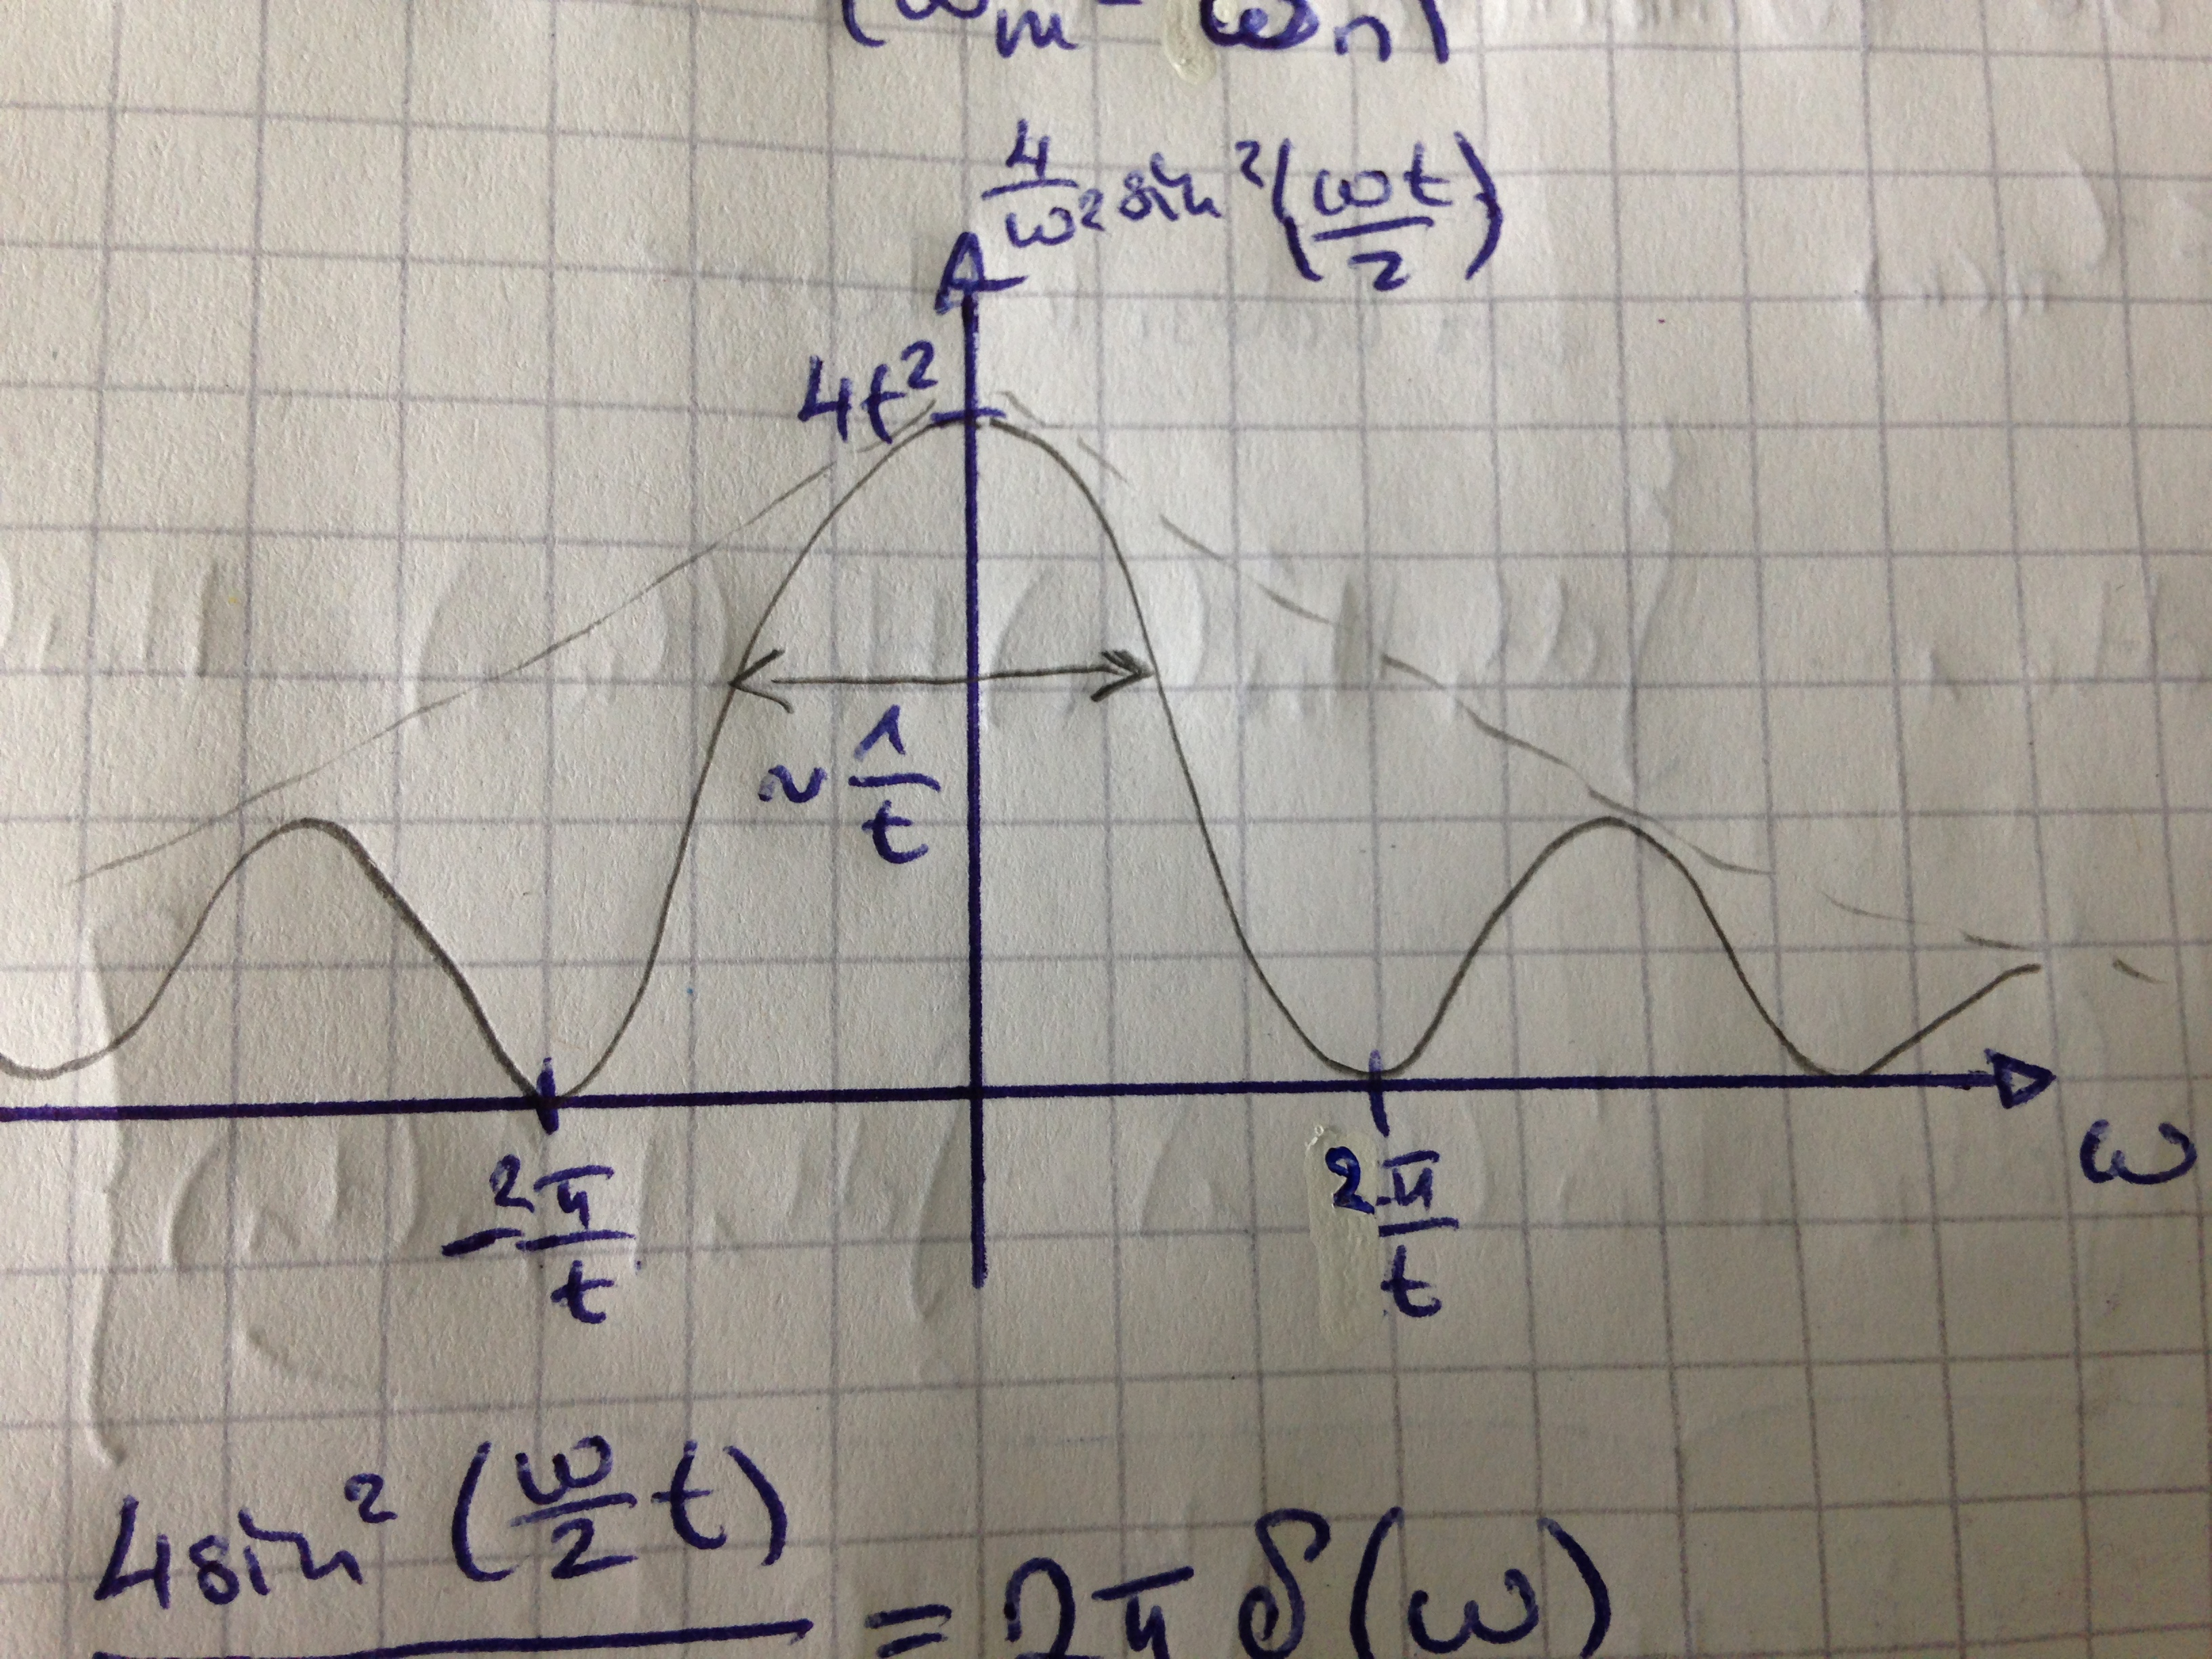
\includegraphics[width=10cm]{Ersatzgraph1.jpg}
		\end{center}
	\end{figure*}
		\begin{equation*}
			\lim\limits_{t \rightarrow \infty} \frac{4 \sin^2(\frac{\omega}{2} t)}{\omega^2 t} = 2 \pi \delta (\omega)
		\end{equation*}
	Annahme $\ket{m} = \ket{\alpha}$ liegt im Kontinuierlichen Teil des Spektrums von $H^0$. Beispiel H-Atom mit
		\begin{align*}
			E_n &= - \frac{1}{2} \frac{m c^2 \alpha^2}{n^2} &
			\ket{\alpha} \text{nicht normiert} \\
			E_{\alpha 0} &\leq E_\alpha \leq E_{\alpha 1}
		\end{align*}
	EINE ZEICHNUNG
	\begin{figure*} [h]
		\begin{center}
			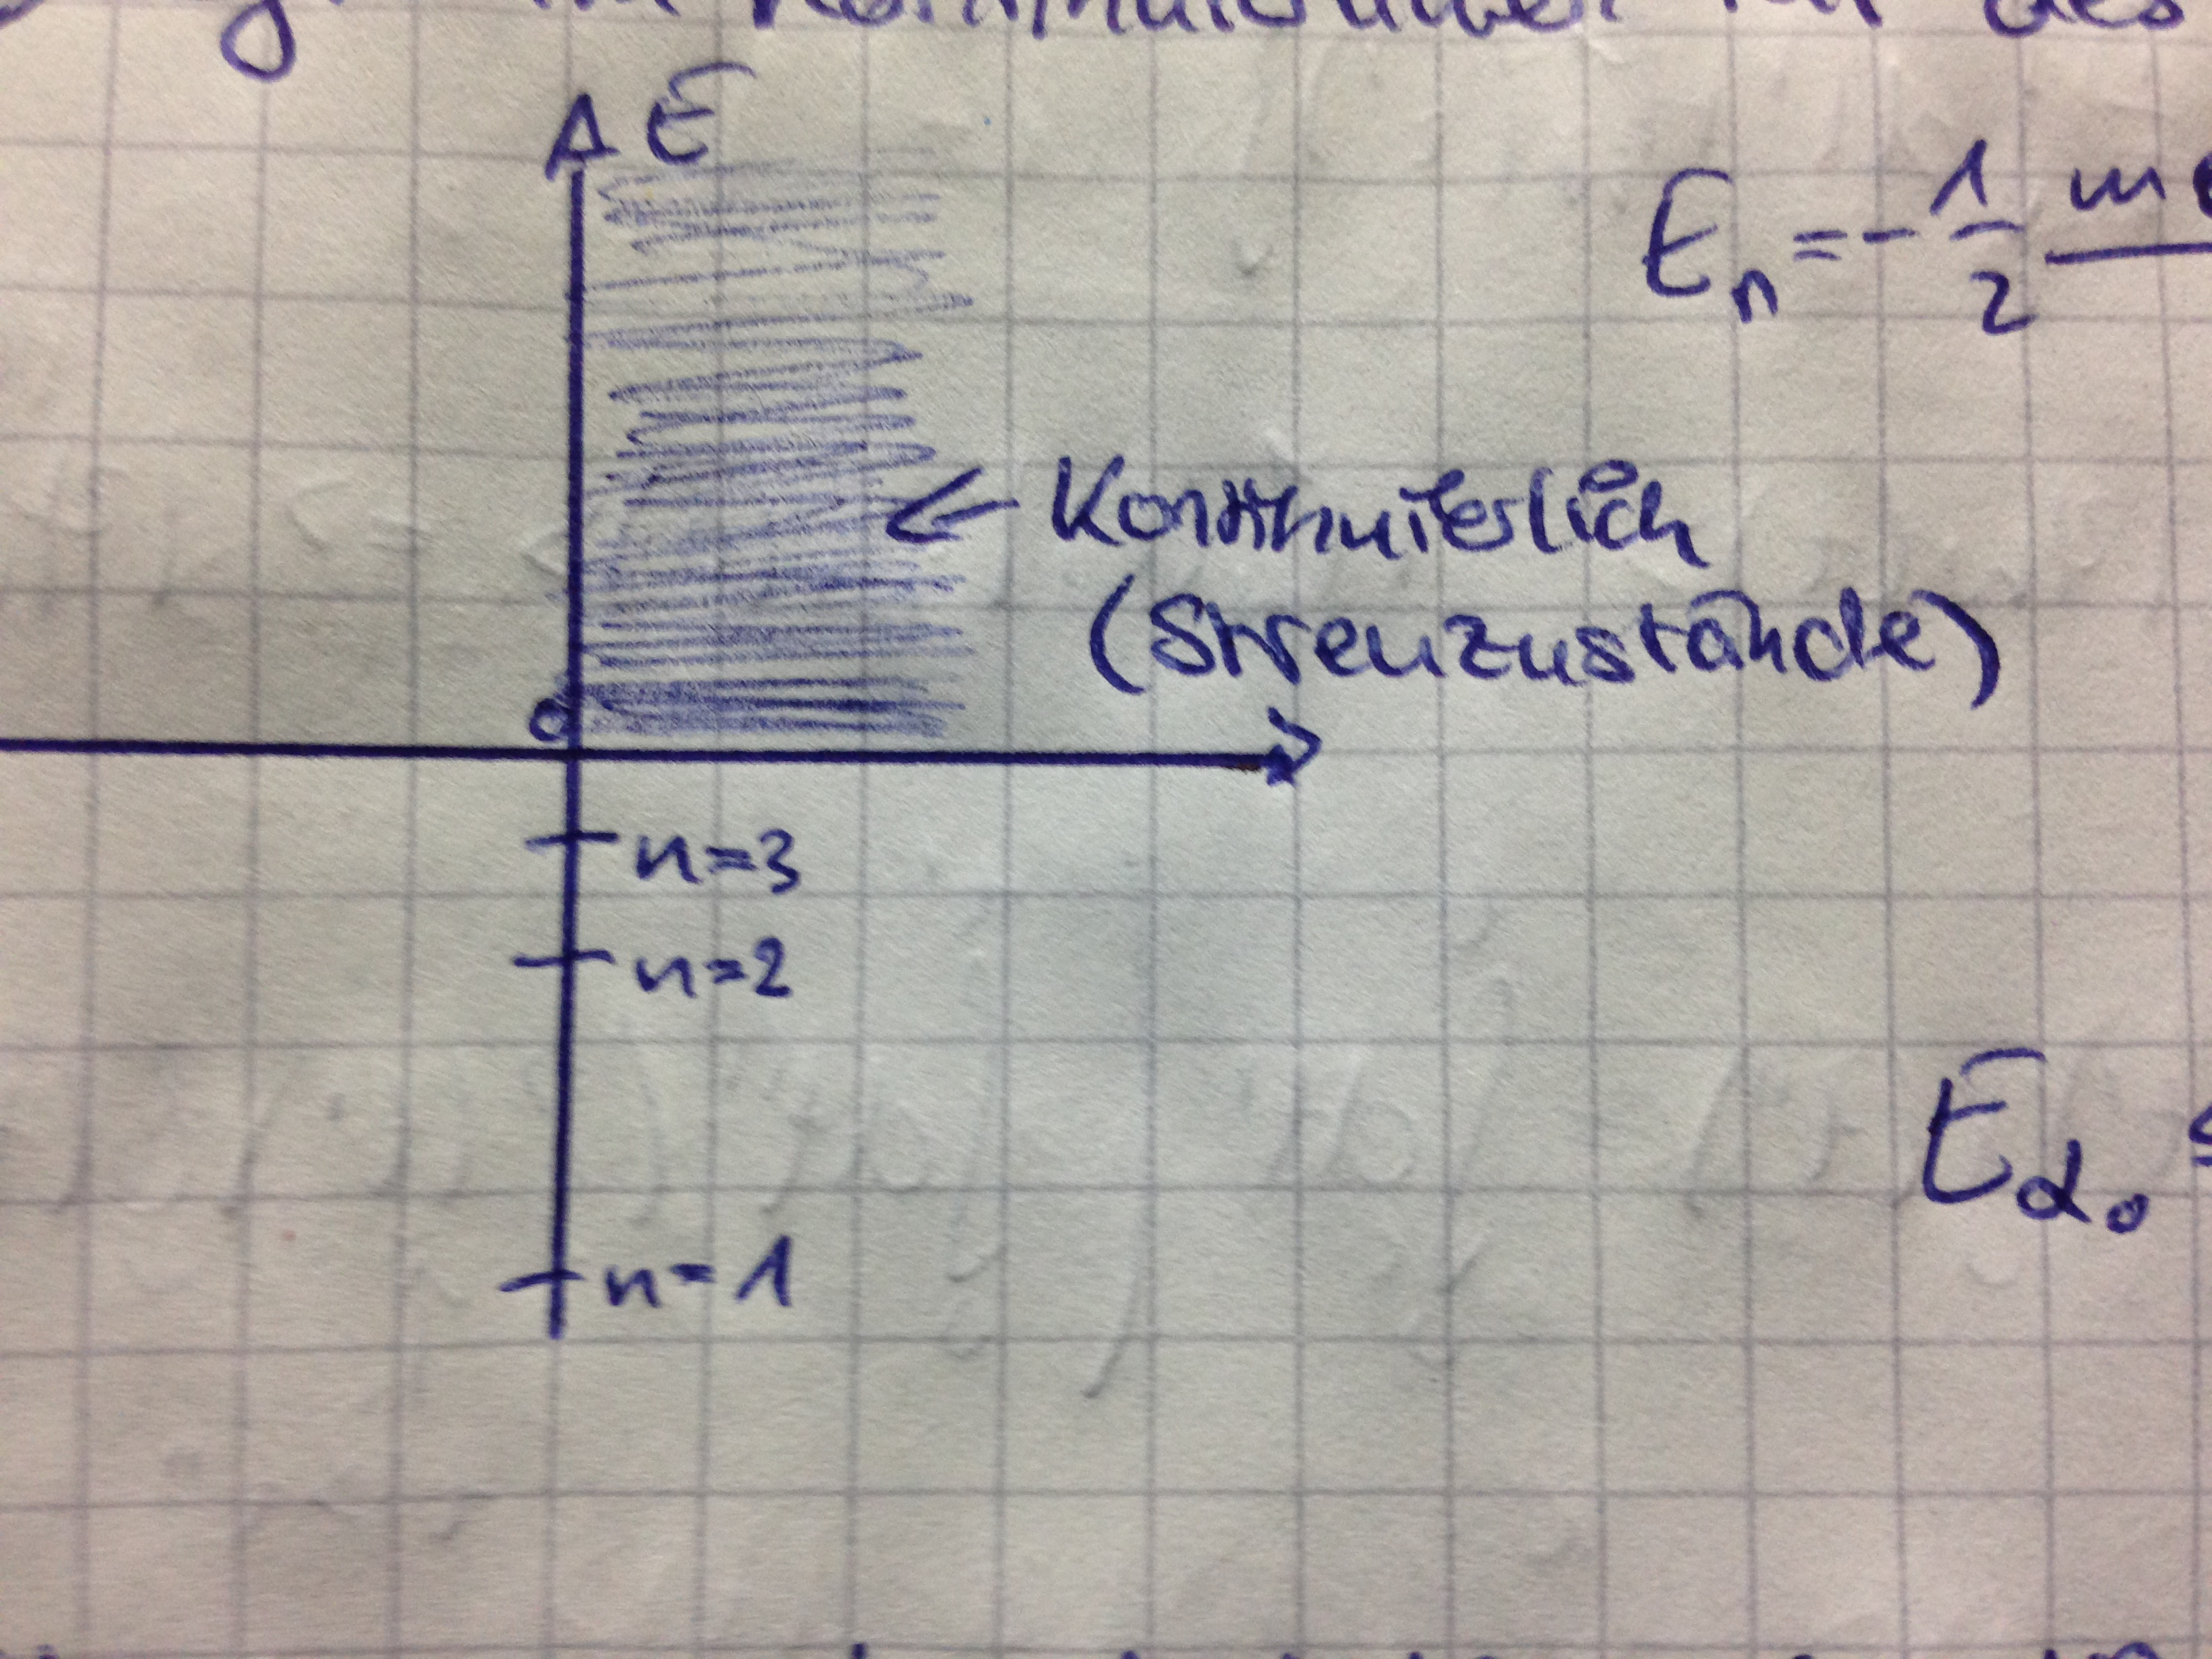
\includegraphics[width=10cm]{Ersatzgraph2.jpg}
		\end{center}
	\end{figure*}

	$P_{\alpha n}(t)$ ist Übergangswahrscheinlichkeits\underline{dichte}
	
	Übergangswahrscheinlichkeit: 
		\begin{equation*}
			\int_{\alpha_0}^{\alpha_1} \diff \alpha P_{\alpha n} (t)
		\end{equation*}
	Übergangsrate (Übergangswahrscheinlichkeit pro Zeiteinheit)
		\begin{align*}
			\underbrace{W_{\alpha \leftarrow n}}_{
				\mathclap{\text{Übergangsrate von~} n \text{~nach~} \alpha}}
			&= \int \diff \alpha \frac{P_{an}(t)}{t} \\
			&\underset{t \rightarrow \infty}{=} 
			\int \diff \alpha \frac{2 \pi}{\hbar^2} 
			\delta(\omega_\alpha - \omega_n) \left| \braket{m | H^1 | n}\right|^2 \\
			&= \int \diff \alpha \frac{2 \pi}{\hbar} 
			\delta (E_\alpha - E_n) \left| \braket{\alpha | H^1 | n}\right|^2
		\end{align*}
	(hier meinte Herr Prof. Bali mit einem Pfeil auf $E_\alpha$: Zeitunabhängige Störung erzwingt Energieerhaltung)
	
	Dichte von Zuständen:
		\begin{align*}
			\rho &= \int \diff \alpha \delta (E_\alpha - E)  \\
			\diff \alpha &= \rho(E_\alpha) \diff E_\alpha: \text{~Zahl der Zustände im ``Ìntervall''~} \diff E_\alpha
		\end{align*}
		\begin{align*}
			\boxed{
				W_{\alpha \leftarrow n} = \frac{2 \pi}{\hbar} \rho(E_n)
					\left| \braket{\alpha | H^1 | n}\right|^2
				}
			\text{~Fermis ``Goldene Regel'' (Wenzel)}
		\end{align*}
	Probleme bei 
		\begin{itemize}
			\item $t$ sehr groß $\Rightarrow \int \diff \alpha P_{\alpha n} > 1$.
			\item $t  << \frac{1}{|\omega_\alpha - \omega_n|}$ (keine $\delta$- Funktion)   
		\end{itemize}	
	Gültigkeitsbereich:
		\begin{itemize}
			\item $\Delta E$ Verteilung der Endzustände muss größer sein als die Breite von $\frac{\sin^2 (\frac{1}{2}(\omega_\alpha - \omega_n) t)}{(\omega_\alpha - \omega_n)^2}$. Damit $\delta$- Funktionsapproximation gerechtfertigt ist, muss $t \gg \frac{2 \alpha \pi}{\Delta E}$ (Version der Unschärferelation)
			\item $t$ muss klein genug sein, damit 1.Ordnung Störungstheorie gerechtfertigt ist:
			\\ $t \ll \frac{1}{W_{\alpha \leftarrow n}}$
		\end{itemize}
		
\subsection{Periodische Störungen}
		\begin{align*}
			H^1(t) &= \left[H_\omega e^{-i \omega t} + H^\dagger_\omega e^{i \omega t}\right]
			\Theta(t) ,& \omega &> 0 \\
			H^{1 \dagger}(t) &= H^1(t) &\Rightarrow H^1(t) &= 0 \text{~für~} t < 0 
		\end{align*}
		\begin{align*}	
			c_m(t) - \delta_{mn} &= - \frac{i}{\hbar} \int_{0}^{t'} \diff t'
			\left\{ \braket{m | H_\omega | n} e^{i (\omega_m - \omega_n - \omega) t'} +
			\braket{m | H_\omega^\dagger | n} e^{i (\omega_m - \omega_n + \omega) t'}
			\right\} + \ldots \\
			\marginnote{Zitat Balis: jetzt bekommen wir hier viele Sinüsse. XD}
			&= - \frac{i}{\hbar} 
			\left\{ \braket{m | H_\omega | n} 
				\frac{\sin \left[\frac{1}{2} (\omega_m - \omega_n + \omega) t 
					\right]}{\frac{1}{2} (\omega_m - \omega_n + \omega)}
				e^{\frac{i}{2} (\omega_m - \omega_n - \omega) t} ~+ \right. \\
			&+ \left. \braket{m | H_\omega^\dagger | n}
				\frac{\sin \left[\frac{1}{2} (\omega_m - \omega_n - \omega) t 
					\right]}{\frac{1}{2} (\omega_m - \omega_n - \omega)}
				e^{\frac{i}{2} (\omega_m - \omega_n + \omega) t}	
			\right\} \\
		\end{align*}
		\begin{align*}
			\Rightarrow \left|c_m(t) - \delta_{mn}\right|^2 
			&= \frac{1}{\hbar^2} 
			\left\{ \left|\braket{m | H_\omega | n}\right|^2
				\frac{4 \sin^2 \left( \frac{1}{2} \left( \omega_{mn} - \omega\right) t
				\right)}{(\omega_{mn} - \omega)^2} ~+ \right. \\
			&+ \left. \left|\braket{m | H^\dagger_\omega | n}\right|^2
			\frac{4 \sin^2 \left( \frac{1}{2} \left( \omega_{mn} + \omega\right) t
				\right)}{(\omega_{mn} + \omega)^2}
			+ \text{gemischte Terme}
			\right\}
		\end{align*}
	mit $\omega_{mn} = \omega_m - \omega_n$
	
		\begin{figure*} [tbp]
			\begin{center}
				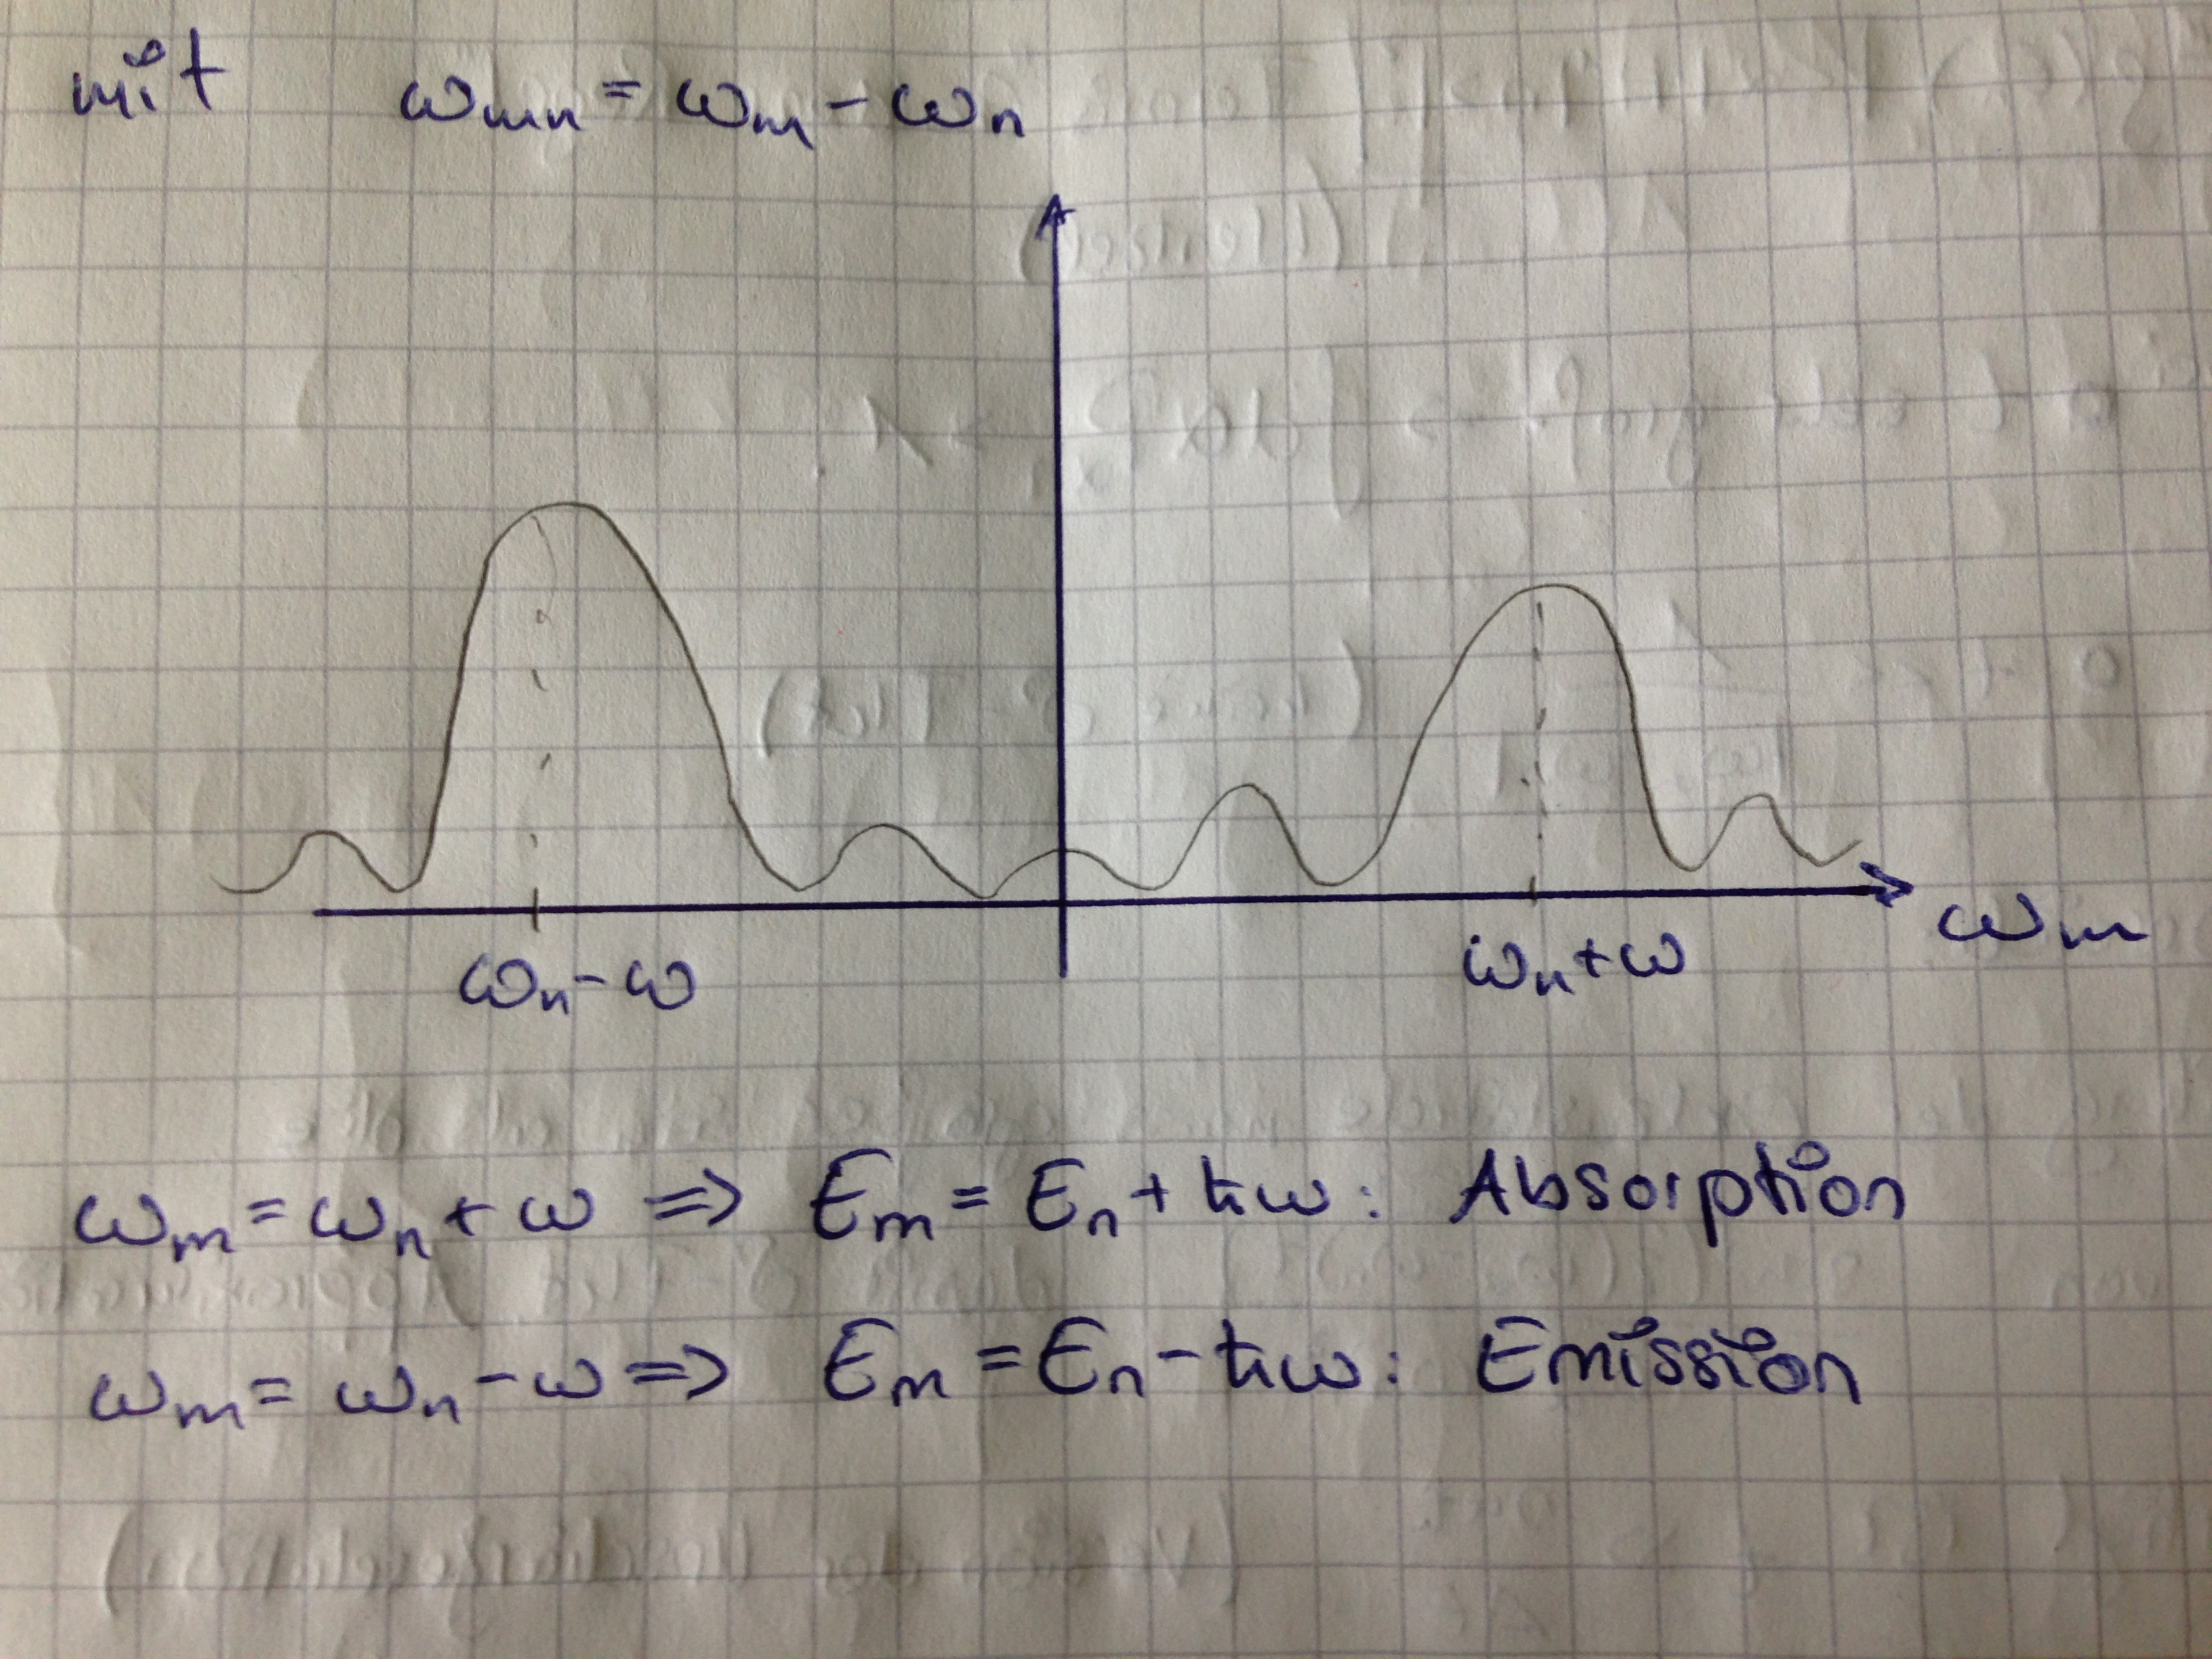
\includegraphics[width=10cm]{Ersatzgraph3.jpg}
			\end{center}
		\end{figure*}
	HIER GRAPH EINFÜGEN
	\FloatBarrier
		\begin{align*}
			\omega_m &= \omega_n + \omega &\Rightarrow E_m &= E_n + \hbar \omega: \text{Absorption} \\
			\omega_m &= \omega_n - \omega &\Rightarrow E_m &= E_n - \hbar \omega: \text{Emission}
		\end{align*}
	\nopagebreak